%!TEX root = ../../../adrien_gomar_phd.tex

In this second example, the linear advection toy problem 
defined in Sec.~\ref{sec:toy_convection} is used with
a perturbation 
in the form of a finite sum of sine functions, similar to the one used
in Sec.~\ref{sec:hb_operator},
applied at the left boundary:
\begin{equation}
    u_l(t) = \cos(\omega t) + \sin(2 \omega t) +
    \cos(3 \omega t) + \sin(4 \omega t) + \cos(5 \omega t).
    \label{eq:sum_injected_fct}
\end{equation}
Harmonic balance computations are run with 1 to 10~harmonics.
For each computation, we show spatial distributions of the solution
at three time instances, namely, $t=0$, $t=T/3$ and $t=2T/3$.
Since these instances are not necessarily used in the HB discretization,
a temporal interpolation is performed.
To do so, the frequency content of the HB solution is used
together with an inverse Fourier transform on the time-vector
$[0, T/3, 2T/3]$.
Figure~\ref{fig:inj_sine_results} depicts the results of HB computations
using 1 to 6~harmonics. The analytical solution is also reported for comparison.

\begin{figure}[htp]
  \centering
  \subfigure[$N=1$]{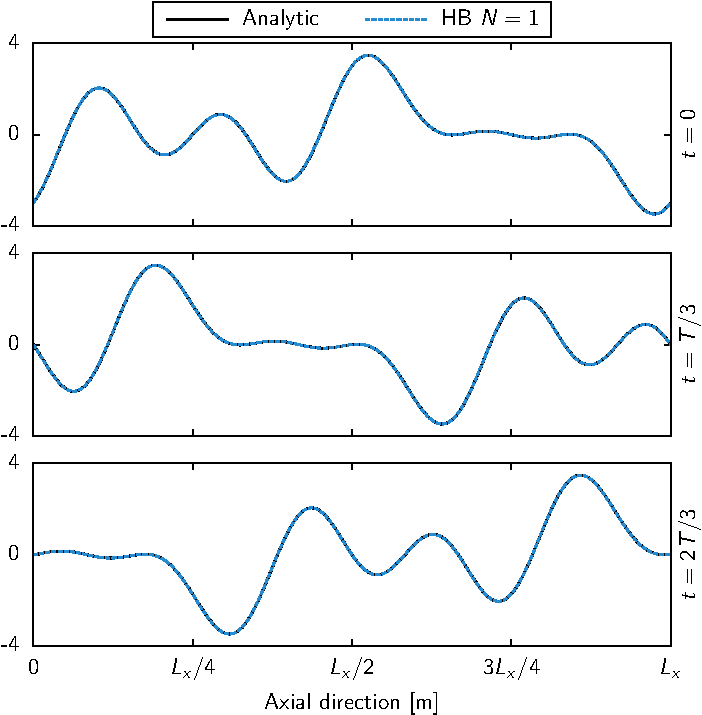
\includegraphics[width=.35\textwidth]{convection_sin_N1.pdf}}
  \subfigure[$N=2$]{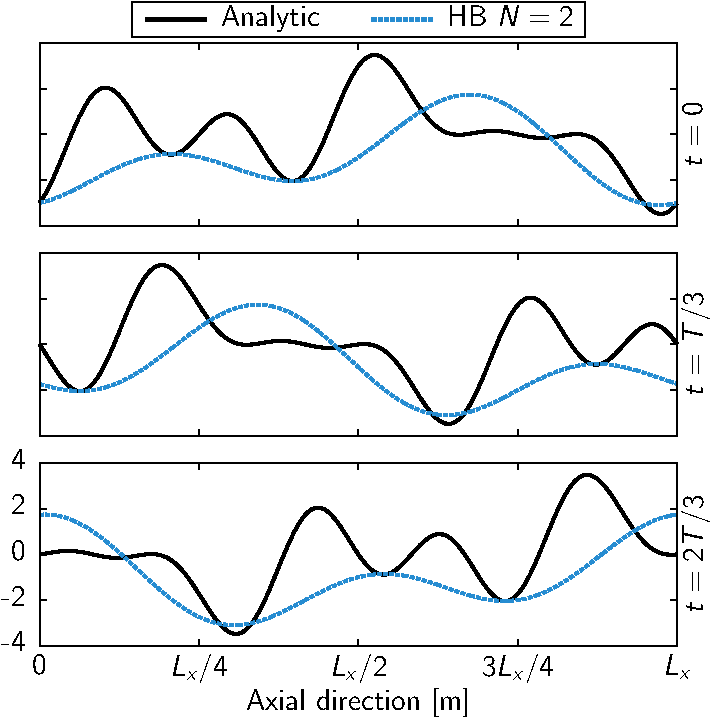
\includegraphics[width=.35\textwidth]{convection_sin_N2.pdf}}
  \subfigure[$N=3$]{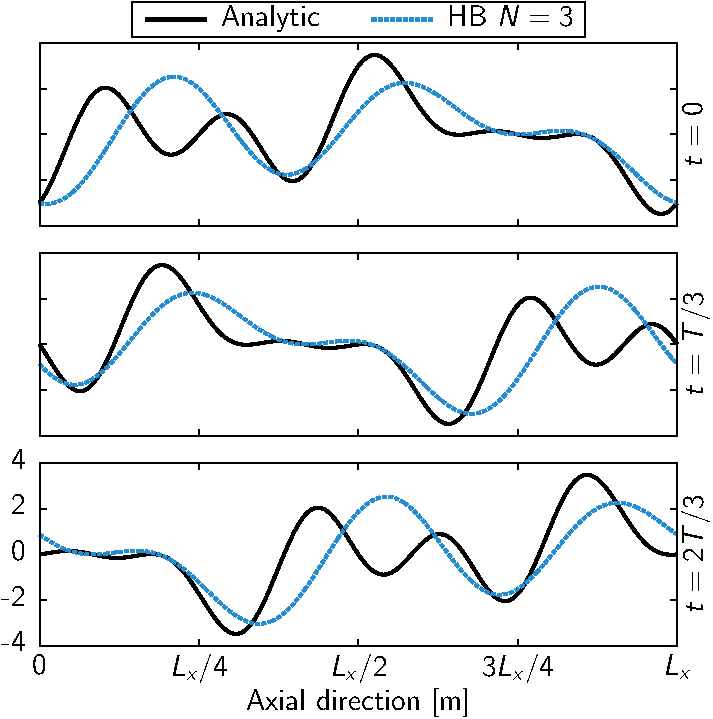
\includegraphics[width=.35\textwidth]{convection_sin_N3.pdf}}
  \subfigure[$N=4$]{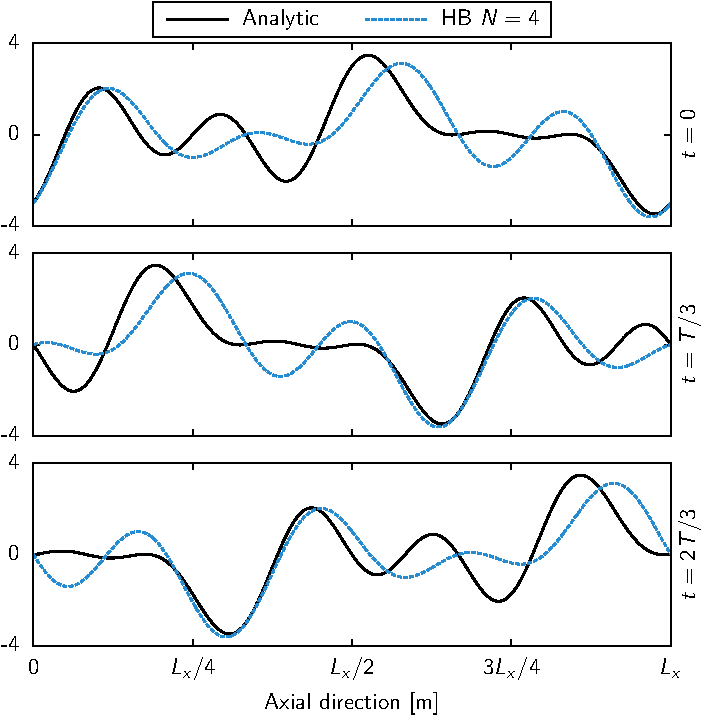
\includegraphics[width=.35\textwidth]{convection_sin_N4.pdf}}
  \subfigure[$N=5$]{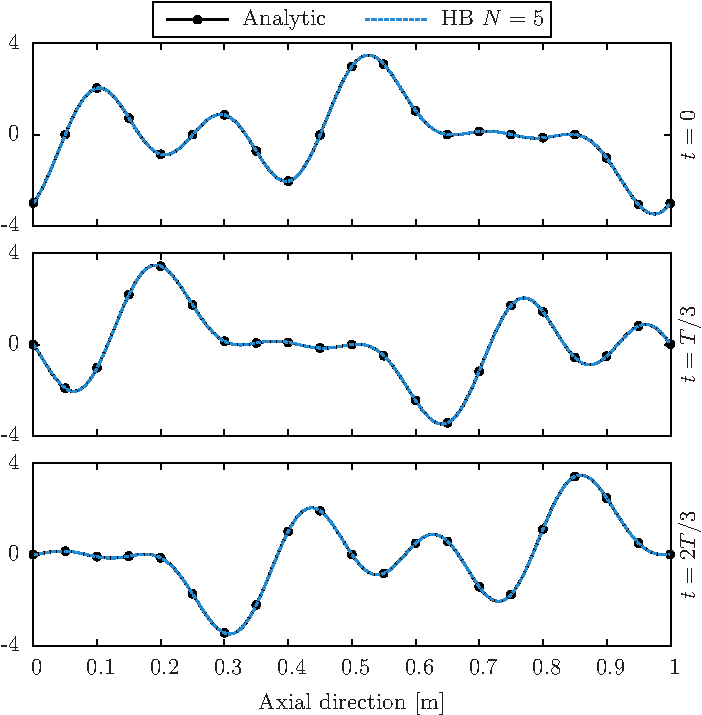
\includegraphics[width=.35\textwidth]{convection_sin_N5.pdf}}
  \subfigure[$N=6$]{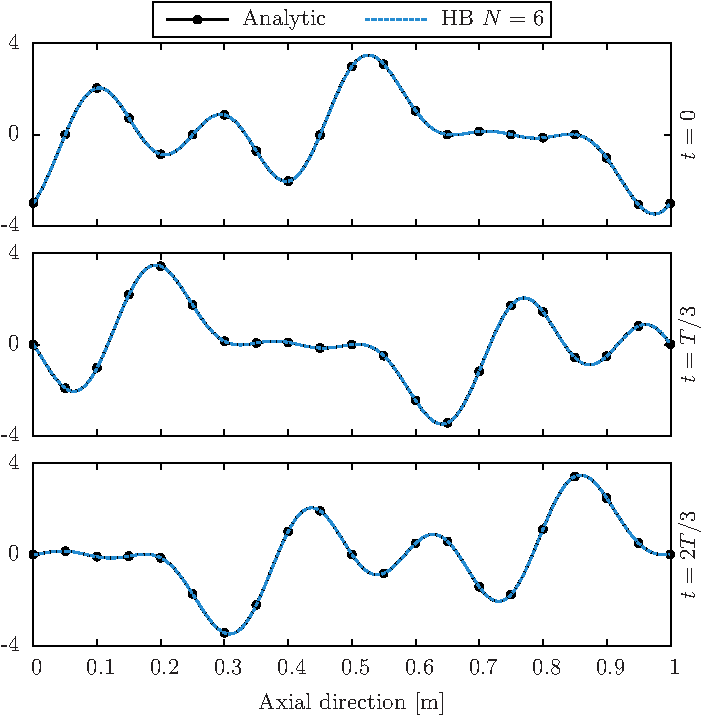
\includegraphics[width=.35\textwidth]{convection_sin_N6.pdf}}
  \caption{Linear advection of a sum of sine functions: 
  numerical solutions at different time instances for different numbers of harmonics.}
  \label{fig:inj_sine_results}
\end{figure}

The accuracy of the solution 
improves with the number of harmonics,
until it reaches the frequency content
of the injected signal, \emph{i.e.} 5~harmonics.
For higher sampling levels, the results of HB computations are
superimposed with the analytical solution. 

The $\mathcal{L}_2$-norm of the error as a function of the number of harmonics
is shown in Fig.~\ref{fig:conv_sum_sine}. Two results are displayed:
one for the reference mesh (2,000 grid points) and one for
a refined mesh (4,000 grid points).
\begin{figure}[htp]
  \centering
  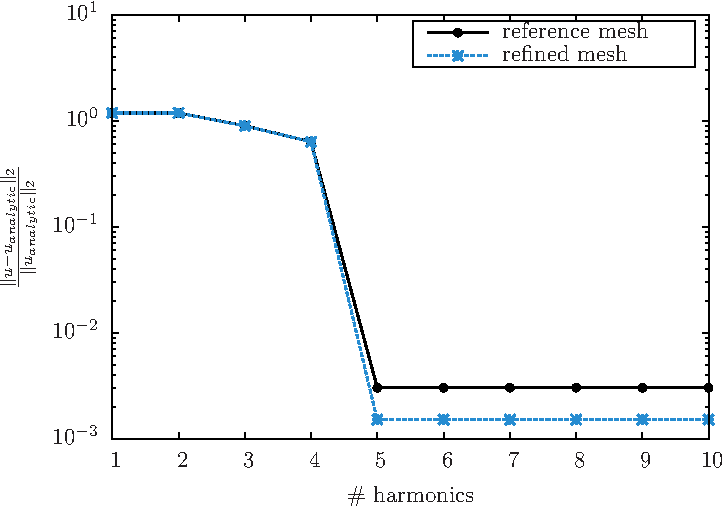
\includegraphics[width=.5\textwidth]{convection_sin_error.pdf}
  \caption{Linear advection of a sum of sine functions: convergence of the HB method error.}
  \label{fig:conv_sum_sine}
\end{figure}
The convergence of the HB computations is slow  for
$N \leq 4$. However, when the number of harmonics composing
the injected function is reached ($N=5$), the error is minimum and computing
more harmonics does not change the error.
The convergence rate 
of Fourier-based time methods is inherently linked to the spectrum of the
temporal phenomenon that one wants to capture. Here a finite discrete spectrum composed of only five harmonics
is imposed.
The value of the plateau obtained 
after $N=5$ is representative of the error introduced by the different
discretizations. In fact, refining the mesh changes this value
without modifying the error levels of the lower harmonics points.

The temporal discrete Fourier transform
of the computational results is compared to the
analytical results in Fig.~\ref{fig:dft_sin}.
\begin{figure}[htp]
  \centering
  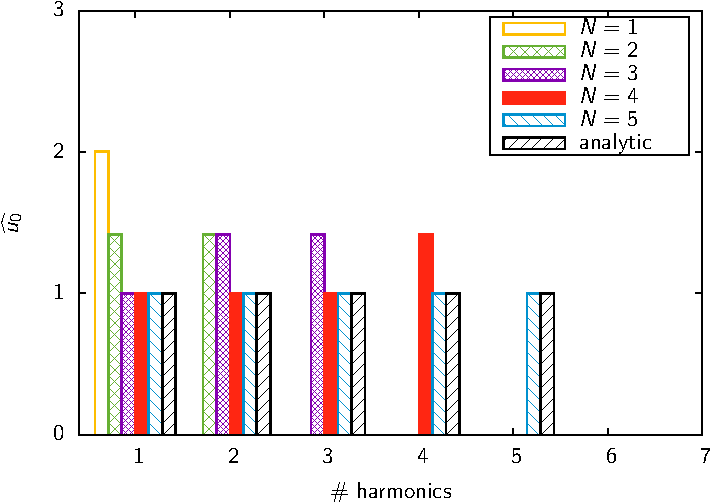
\includegraphics[width=.5\textwidth]{convection_sin_dft.pdf}
  \caption{Linear advection of a sum of sine functions: 
  discrete Fourier transform.}
  \label{fig:dft_sin}
\end{figure}
When the number of harmonics grows in the spectral computations,
the Fourier transform gets closer to the analytical solution.
When the whole frequency content of the injected 
function is contained in the HB solution, 
the numerical results are superimposed with the analytical ones.
For intermediate sampling frequencies, as for 
instance the three-harmonics HB computation, 
the resolved harmonics have higher amplitudes 
than the exact one, since they compensate for harmonics that are not resolved.

When the number of harmonics composing the spectrum of the
computed signal is reached, the computational results are superposed
with the analytical ones to with plotting accuracy, namely we obtain spectral accuracy.
This is the main advantage of Fourier-based time methods: when the
signal has a narrow spectrum, as it is the case for the sum
of sine function used here, the
convergence can be very fast compared to a classical time-marching scheme
as only a few number of time instances is necessary to retrieve the
unsteadiness.

